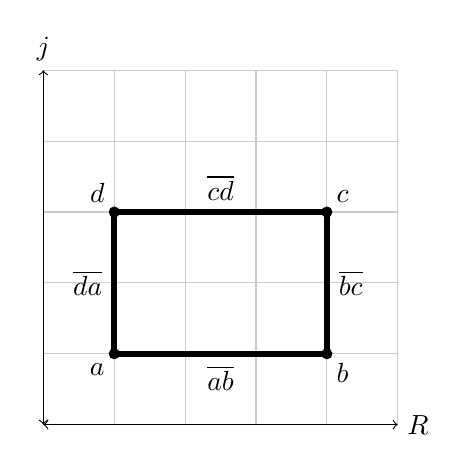
\begin{tikzpicture}[scale=0.9]
    \draw[thin,gray!40] (0,0) grid (5,5);
    \draw[<->] (0,0)--(5,0) node[right] {$R$};
    \draw[<->] (0,0)--(0,5) node[above]{$j$};
    \coordinate (1) at (1,1);
    \coordinate (2) at (4,1);
    \coordinate (3) at (4,3);
    \coordinate (4) at (1,3);
    
    \draw[fill=black] (1) circle(2pt) node[anchor=north east]{$a$};
    \draw[fill=black] (2) circle(2pt) node[anchor=north west]{$b$};
    \draw[fill=black] (3) circle(2pt) node[anchor=south west]{$c$};
    \draw[fill=black] (4) circle(2pt) node[anchor=south east]{$d$};
    
    \draw[line width=2pt,black,-] (1)--(2) node[midway, below]{$\overline{ab}$};
    \draw[line width=2pt,black,-] (2)--(3) node[midway, right]{$\overline{bc}$};
    \draw[line width=2pt,black,-] (3)--(4) node[midway, above]{$\overline{cd}$};
    \draw[line width=2pt,black,-] (4)--(1) node[midway, left]{$\overline{da}$};
    
\end{tikzpicture}
\caption*{Rectángulo $s$}
